\documentclass[12pt]{article}
\usepackage{graphicx}
\usepackage[utf8]{inputenc}
\usepackage[english]{babel}
\usepackage{fullpage}
\usepackage{listings}
\usepackage{xcolor}
\usepackage{url}
\usepackage[linesnumbered,ruled,vlined]{algorithm2e}
\usepackage{enumitem}
\usepackage{mathrsfs}
\usepackage{amssymb}
\usepackage{amsmath}
\usepackage{enumitem}
\usepackage{hyperref}
\usepackage{float}
\usepackage{sbc-template}


\definecolor{mygreen}{rgb}{0,0.6,0}

\hypersetup{
    colorlinks=true,
    linkcolor=cyan,
    urlcolor=cyan}

\newcounter{problem}
\newcounter{solution}

\pagestyle{plain}
\thispagestyle{plain}

\newtheorem{ex}{Exemplo}[section]
\newtheorem{theorem}{Teorema}
\newtheorem{corollary}{Corolário}[theorem]
\newtheorem{lemma}[theorem]{Lemma}
\newtheorem{definition}{Definição}

\lstset{ % lstlisting
    language=Python,
    frame=tb, % draw a frame at the top and bottom of the code block
    tabsize=4, % tab space width
    showstringspaces=false, % don't mark spaces in strings
    commentstyle=\color{mygreen}, % comment color
    keywordstyle=\color{blue}, % keyword color
    stringstyle=\color{red}, % string color
    numbers=left, 
    numbersep=9pt,
    backgroundcolor=\color{black!5}, % set backgroundcolor
    basicstyle=\footnotesize,% basic font setting
}

\newcommand\Problem{%
  \stepcounter{problem}%
  \textbf{Problema \theproblem:}
  \setcounter{solution}{0}%
}

\newcommand\TheSolution{%
  \textbf{Solução:}\\%
}

\newcommand\ASolution{%
  \stepcounter{solution}%
  \textbf{Solução \thesolution:}\\%
}
% \parindent0in
\parskip 1.5em

\title{Curso de Curvas e Superfícies}

\author{Wellington José Leite da Silva\inst{1}}

\address{Escola de Matemática Aplicada da FGV (EMAP), Brazil}

\date{}

\begin{document}

\maketitle


\section*{Indrodução}\label{s1}
Apresentamos aqui a linha de aprendizado do curso de curvas e superfícies apresentando definições, teoremas e etc. Seguindo principalmente o livro \cite{bookmain} e adicionando sempre que possível, exemplos ilustrativos usando o \textit{sagemath}. As implementações apresentadas aqui também estão presentes num \textit{jupyter-notebook} no \href{https://github.com/wellington36/curvas-superficies/blob/main/Jupyter_auxiliary.ipynb}{github}.

Para os códigos apresentados aqui, usamos a biblioteca \textit{utils} que está no \href{https://github.com/wellington36/curvas-superficies/blob/main/utils.py}{github} e habilitamos a exibição de LaTeX, como apresentado no \textit{jupyter-notebook} mencionado acima.

\section{Curvas, Reta tangente e Comprimento de arco}\label{s2}

\begin{definition}
Uma \textbf{curva parametrizada} $\alpha$ em $\mathbb{R}^n$ é uma aplicação $\gamma: I \rightarrow \mathbb{R}^n$ sendo $I \subset \mathbb{R}$ aberto, da forma

$$\alpha(t) = (x(t), y(t)),\ t\in I$$

onde x e y são funções diferenciáveis de t.
\end{definition}

\begin{ex}[Curva parametrizada diferenciável] A curva $\alpha(t) = (4/5 \sin(t), - cos(t))$ é um exemplo de curva parametrizada diferenciável e define uma elipse
\begin{lstlisting}
# curve definition
curve_alpha(t) = (1/2 * cos(t) + 1/3 * sin(4 * t), 
                  1/2 * sin(t) + 1/3 * cos(4 * t))

# plot
parametric_plot(curve_alpha, (t,0, 2*pi), thickness=2)
\end{lstlisting}

\begin{figure}[H]
    \centering
    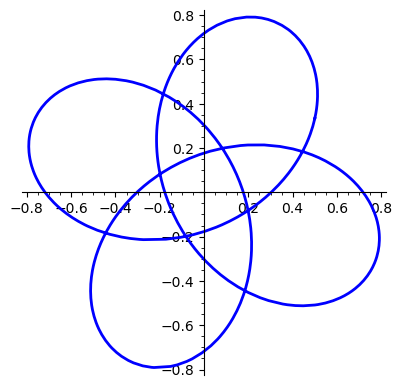
\includegraphics[scale=.6]{Images/ex1.1.png}
    \caption{Curva parametrizada}
    \label{fig:ex1.1}
\end{figure}
\end{ex}

\begin{definition}
O conjunto imagem de uma curva $\gamma$, $\gamma(I) \subset \mathbb{R}^n$ é dito o \textbf{traço} de $\gamma$.
\end{definition}

\begin{definition}[Vetor tangente]
Seja $\gamma: I \rightarrow \mathbb{R}^n$ com $\gamma(t) = (\gamma_1 (t), \ldots, \gamma_n (t))$ com $\gamma_i (y)$ diferenciáveis $\forall i, i = 1 \ldots n$, o vetor

$$\gamma'(t) = (\gamma'_1 (t), \ldots, \gamma'_n (t))$$

é chamado \textbf{vetor tangente de $\gamma$} em t
\end{definition}

\begin{ex}[Vetores tangentes] Usando a mesma curva acima podemos visualizar os vetores tangentes da seguinte forma
\begin{lstlisting}
M = Manifold(2, 'M')
X.<x,y> = M.chart()

c = M.curve([1/2 * cos(t) + 1/3 * sin(4 * t), 
             1/2 * sin(t) + 1/3 * cos(4 * t)], (t, 0, 2*pi))

v = c.tangent_vector_field() ; v

show(c.plot(thickness=2, aspect_ratio=1) +
     v.plot(chart=X, number_values=30, scale=.2))
\end{lstlisting}

\begin{figure}[H]
    \centering
    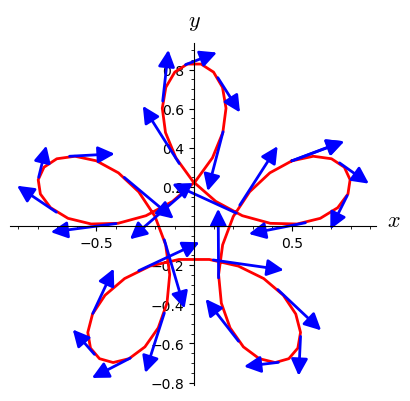
\includegraphics[scale=.6]{Images/ex1.2.png}
    \caption{Vetores tangentes}
    \label{fig:ex1.2}
\end{figure}

\end{ex}

\begin{definition}[Curvas regulares]
Seja $\gamma (t): I \rightarrow \mathbb{R}^n$ uma curva parametrizada diferenciável. Diz-se que \textbf{$\gamma$ é regular}, quando $\gamma'(t) \neq 0,\ \forall t \in I$.
\end{definition}

\begin{definition}[Comprimento de arco]
O \textbf{comprimento de arco de $\alpha$}, de $\alpha(a)$ até $\alpha(b)$ definido por $L_a^b (\alpha)$ é  

$$L_a^b (\alpha) = \int_a^b \| \alpha'(t) \| d t$$
\end{definition}

\begin{ex}[Comprimento de arco] O comprimento de arco da curva $\alpha(t) = (2 \cos(t), 2 \sin(t))$ pode ser encontrada fazendo
\begin{lstlisting}
curve_alpha(s) = (2 * cos(s), 2 * sin(s))

x = get_vector_arguments(curve_alpha).pop()
curve_alpha_x = curve_alpha.derivative(x)
    
# Calcular comprimento de arco de 0 a t
t = var("t")
assume(t>0)
s = integrate(norm(curve_alpha_x), (x,0,t))
s = s.simplify_full()

pretty_results((r"\int_0^t || C'(x) || dx", s))
\end{lstlisting}

\newcommand{\Bold}[1]{\mathbf{#1}}\begin{align*} \int_0^t || C'(x) || dx &= 2t \\ \end{align*} \\
\end{ex}

\begin{definition}
Se $\gamma: (a, b) \rightarrow \mathbb{R}^n$ é uma c.p.\footnote{curva parametrizada}, sua \textbf{velocidade no ponto} $\gamma(t)$ é $\| \gamma'(t) \|$, e a curva é dita com \textbf{velocidade unitária} se $\| \gamma'(t) \| = 1,\ \forall t \in (a, b)$ e é parametrizada por comprimento de arco.
\end{definition}

\begin{theorem}
Toda \textbf{curva regular} pode ser reparametrizada por \textbf{comprimento de arco}.
\end{theorem}

\bibliographystyle{sbc}
\bibliography{referencias}

\end{document}